% !TeX spellcheck = si_SI
% Predloga za pisanje zaključnih nalog, LADISK 2015-2017, pripravil Martin Česnik, Janko Slavič
% Zadnja verzija na: https://github.com/ladisk/latex-templates
\documentclass[12pt,a4paper,twoside,fleqn,openright]{book}

% use quite a lot of packages
\usepackage{amsfonts,amssymb,amsmath}
\usepackage{enumerate}
\usepackage[section]{placeins}
\usepackage{float}
\usepackage[slovene]{babel}
\usepackage[utf8]{inputenc}
\usepackage{graphicx}
\usepackage{notoccite}
\usepackage{ifthen}
\usepackage{fancyhdr}
\usepackage{longtable}
\usepackage{hyperref}
\usepackage{ifoddpage}
\usepackage{tocloft}
\usepackage{titlesec}
\usepackage{pdfpages}
\usepackage{nameref}
\usepackage{multirow}
\usepackage{caption}
\usepackage{subcaption}
\usepackage{enumitem}
\usepackage[numbib]{tocbibind}
\usepackage{url}
\usepackage{cite}
\usepackage[inner=30mm,
            outer=25mm,
            top=30mm,
            bottom=25mm]{geometry}

% paragraph settings
\setlength\parindent{0pt}
\setlength{\parskip}{1.5ex plus 0.5ex minus 0.5ex}

% set equation environment indentation
\setlength{\mathindent}{0.5cm}%

% set itemize environment whitespacing and left margin
\setlist[itemize]{noitemsep,nolistsep, leftmargin=*}

% set table and figure captions
\captionsetup[table]{skip=10pt,singlelinecheck=false}
\captionsetup[figure]{justification=centering}

% set tablename to Preglednica
\AtBeginDocument{%
  \renewcommand\tablename{Preglednica}
}

% command for multiline cell in table
\newcommand{\minitab}[2][l]{\begin{tabular}{#1}#2\end{tabular}}

% opens a new page if current page is even
\newcommand{\addifeven}{
\checkoddpage
\ifoddpage
\else
\mbox{}
\newpage
\fi}

% set section and tableofcontents depth
\setcounter{secnumdepth}{3}
\setcounter{tocdepth}{3}
\def\labelitemi{--}

%  accordingly format a chapter definition
\titleformat{\chapter}[display]
  {\bfseries}{}{0pt}{\Huge\thechapter\quad}


% set fancy_nohead fancy header
\fancypagestyle{fancy_nohead}{
\fancyfoot[LE,RO]{\thepage}
\fancyhead{}
\renewcommand{\headrulewidth}{0pt}
\chead{}
\cfoot{}
}

% assign no_header
\assignpagestyle{\chapter}{fancy_nohead}

% section and chapter formatting
\renewcommand{\thechapter}{\arabic{chapter}.}
\renewcommand{\thesection}{\arabic{chapter}.\arabic{section}.}
\renewcommand{\thesubsection}{\thesection\arabic{subsection}.}
\renewcommand{\thesubsubsection}{\thesubsection\arabic{subsubsection}.}
\renewcommand{\thetable}{\arabic{chapter}.\arabic{table}}
\renewcommand{\thefigure}{\arabic{chapter}.\arabic{figure}}
\renewcommand{\theequation}{\arabic{chapter}.\arabic{equation}}

\renewcommand\cftchapdotsep{\cftdotsep}  % adds leader dots from chapter titles to page numbers

\begin{document}


\pagenumbering{roman}
% !TeX spellcheck = si_SI
%Urejanje platnic, naslovnice, UDK, povzetka in kazal
%
% PLATNICA
% -*- TeX:SI -*-
% Platnica
\thispagestyle{empty}
\begin{center}
\large \mbox\par\par\vspace*{-0.75cm} \textbf{UNIVERZA V LJUBLJANI}
\\ \vspace{0.2cm} \large{Fakulteta za strojništvo}
\\ \vspace*{6cm} \LARGE{\textbf{[Naslov doktorskega dela na Fakulteti za strojništvo]}}
\\ \vspace{1cm} \normalsize
\large{Doktorsko delo}\\
\vspace{2cm}
\large{Predložil(-a) Fakulteti za strojništvo Univerze v Ljubljani za pridobitev znanstvenega naslova doktor znanosti}\\
\vspace{2.5cm}
\Large{\textbf{[Janez Novak]}}\\
\vfill
\large{Ljubljana, [avgust 2013]}
\end{center} 
\newpage

% TRI PRAZNE STRANI
\mbox{}\thispagestyle{empty}
\newpage
\mbox{}\thispagestyle{empty}
\newpage
\mbox{}\thispagestyle{empty}
\newpage

% NOTRANJA NASLOVNICA
% -*- TeX:SI -*-
% Notranja naslovnica
\thispagestyle{empty}
\begin{center}
\large \mbox\par\par \vspace*{-0.75cm}\textbf{UNIVERZA V LJUBLJANI}
\\ \vspace{0.2cm} \large{Fakulteta za strojništvo}
\\ \vspace*{6.5cm} \LARGE{\textbf{[Zasnova predloge za zaključne naloge na Fakulteti za strojništvo]}}
\\ \vspace{1cm} \normalsize
\large{Zaključna naloga Razvojno raziskovalnega programa I. stopnje Strojništvo}\\
\vspace{2cm}
\Large{\textbf{[Janez Novak]}}\\
\vspace{5cm}
\large{
Mentor: [prof. dr. Franc Horvat, univ. dipl. inž.]\\
Somentor: [prof. dr. Anton Kovačič, univ. dipl. inž.]
}
\vfill
\large{Ljubljana, [avgust 2013]}
\end{center}
\setcounter{page}{1} 
\newpage
\mbox{}\thispagestyle{empty}
\newpage

% PROSTOR ZA ODLOČBO
\thispagestyle{empty}
[Prostor za podpisano temo magistrskega dela]
\newpage
\mbox{}\thispagestyle{empty}
\newpage

% PROSTOR ZA ZAHVALO
\pagestyle{fancy_nohead}
% -*- TeX:SI -*-
% Zahvala
\vspace*{0mm}
\Large\textbf{Zahvala}\normalsize
\vskip\medskipamount % or other desired dimension
\leaders\vrule width \textwidth\vskip0.4pt % or other desired thickness
\vskip\bigskipamount % ditto


[Pisanje zahvale ali posvetila je neobvezno.]\\

[Pri zahvali napišite zahvalo tistim, ki so pomagali pri nastanku dela in brez katerih delo ne bi nastalo v takšni obliki, kot je. Navadno se je potrebno zahvaliti v prvi vrsti mentorju, somentorju in inštituciji, ki je morda finančno ali kako drugače podprla izvedbo zaključnega dela. Nato sledijo asistenti, ostali sodelavci in vaši kolegi, ki so pomagali pri teoretičnem in eksperimentalnem delu. Na koncu se po navadi zahvalimo še družini.]


\newpage
\mbox{}
\newpage

% AVTORSKE PRAVICE
% Podatki o avtorskih pravicah
\vspace*{0mm}
\Large\textbf{Izjava}\normalsize
\vskip\medskipamount % desired skip
\leaders\vrule width \textwidth\vskip0.4pt % desired thickness
\vskip\bigskipamount

\begin{enumerate}[leftmargin=*]
\item Spodaj podpisani(-a) [Janez Novak], rojen(-a) [7. 10. 1989 v Ljubljani], študent(-ka) Fakultete za strojništvo Univerze v Ljubljani, izjavljam, da sem zaključno nalogo z naslovom [Zasnova predloge za zaključne naloge na Fakulteti za strojništvo], izdelal(-a) samostojno v sodelovanju z mentorjem [prof. dr. Francem Horvatom] in somentorjem [prof. dr. Antonom Kovačičem].
\item Izjavljam, da je zaključna naloga, ki sem jo (-ga) oddal(-a) v elektronski obliki, identična tiskani verziji.
\item Izrecno izjavljam, da v skladu z določili Zakona o avtorski in sorodnih pravicah (Ur. l. RS, št. 21/1995 s spremembami) dovolim objavo zaključne naloge na spletnih straneh Fakultete in Univerze v Ljubljani.
\item S podpisom se strinjam z javno objavo svoje zaključne naloge na straneh na svetovnem spletu preko Repozitorija Univerze v Ljubljani.
\end{enumerate}

S svojim podpisom zagotavljam, da:
\begin{itemize}[label={-}]
\item je predloženo besedilo rezultat izključno mojega lastnega raziskovalnega dela;
\item je predloženo besedilo jezikovno korektno in tehnično pripravljeno v skladu z Navodili za izdelavo zaključnih del, kar pomeni, da sem:
\begin{itemize}[label={-}]
\item poskrbel(-a), da so dela in mnenja drugih avtorjev oziroma avtoric, ki jih uporabljam v zaključni nalogi, citirana oziroma navedena v skladu z Navodili za izdelavo zaključnih del, in
\item pridobil(-a) vsa dovoljenja za uporabo uporabljenih podatkov in avtorskih del, ki so v celoti (v pisni ali grafični obliki) uporabljena v tekstu, in sem to v besedilu tudi jasno zapisal(-a);
\end{itemize}
\item se zavedam, da je plagiatorstvo – predstavljanje tujih del (v pisni ali grafični obliki) kot mojih lastnih – kaznivo po Kazenskem zakoniku (Ur. l. RS, št. 55/2008 s spremembami);
\item se zavedam posledic, ki bi jih na osnovi predložene zaključne naloge dokazano plagiatorstvo lahko predstavljalo za moj status na Fakulteti za strojništvo Univerze v Ljubljani v skladu z relevantnim pravilnikom.
\end{itemize}
\vspace{2cm}
V Ljubljani, dne [15.7.2013]\hfill Podpis avtorja(-ice):~\underline{\hspace{4cm}} 
\newpage
\mbox{}
\newpage

% IZVLEČKI IN UDK
% -*- TeX:SI -*-
% UDK in izvlečki
%
%slovenska kodna stran
\vspace*{0mm}
\Large\textbf{Izvleček}\normalsize
\vskip\medskipamount
\leaders\vrule width \textwidth \vskip0.4pt
\vspace{5mm}
\hfill UDK [123.45:678.91:234.56(789.1)]\\
Tek. štev.: [DR III/99]
\par \vspace{1cm}
\large{\textbf{[Naslov doktorskega dela na Fakulteti za strojništvo]}}\normalsize
\par \vspace{1cm}
[Janez Novak]
\par \vspace{1cm}
Ključne besede:
\hspace{1cm}\parbox[t]{10cm}{{[}predloga{]}\\
{[}doktorsko delo{]} \\
{[}navodila{]}\\
{[}vsebina{]}\\
{[}doktoriranje{]}\\
{[}pravilnik{]}}
\par \vspace{3.5cm}


[V začetku izvlečka je jedrnat opis obravnavanega problema. Sledi opis izbrane metodologije in nato opis najpomembnejših rezultatov oz. ugotovitev brez dodatnih pojasnjevanj. Obseg izvlečka naj ne presega 200 besed oz. 600 znakov vključno s presledki.]
\newpage
\mbox{}\newpage
%
%
%angleška kodna stran
\vspace*{0mm}
\Large\textbf{Abstract}\normalsize
\vskip\medskipamount
\leaders\vrule width \textwidth\vskip0.4pt
\vspace{5mm}
\hfill UDC [123.45:678.91:234.56(789.1)]\\
No.: [DR III/99]
\par \vspace{1cm}
\large{\textbf{[Title of doctoral thesis at the Faculty of Mechanical Engineering]}}\normalsize
\par \vspace{1cm}
[Janez Novak]
\par \vspace{1cm}
Key words:
\hspace{1cm}\parbox[t]{10cm}{{[}template{]}\\
{[}doctoral thesis{]} \\
{[}instructions{]}\\
{[}contents{]}\\
{[}graduation{]}\\
{[}regulations{]}}
\par \vspace{3.5cm}


[Angleški prevod izvlečka\ldots]
\newpage
\mbox{}\newpage 
\newpage

% KAZALA
\vspace*{0mm}
\Large\textbf{Kazalo}\normalsize
\vskip\medskipamount
\leaders\vrule width \textwidth\vskip0.4pt
\vskip\bigskipamount

% Vsebinsko kazalo
\makeatletter
\renewcommand{\tableofcontents}{\@starttoc{toc}}
\makeatother
\tableofcontents

\newpage
\addifeven

\vspace*{0mm}
\Large\textbf{Kazalo slik}\normalsize
\vskip\medskipamount
\leaders\vrule width \textwidth\vskip0.4pt
\vskip\bigskipamount

% Seznam slik
\makeatletter
\renewcommand{\listoffigures}{\@starttoc{lof}}
\makeatother
\renewcommand\cftfigpresnum{Slika~}
\renewcommand\cftfigaftersnum{:}

\newlength{\mylen} % a "scratch" length
\settowidth{\mylen}{\bfseries\cftfigpresnum\cftfigaftersnum} % extra space
\addtolength{\cftfignumwidth}{\mylen} % add the extra space
\setlength{\cftfigindent}{0pt}

\listoffigures

\addcontentsline{toc}{section}{Kazalo slik}

\newpage
\addifeven

\vspace*{0mm}
\Large\textbf{Kazalo preglednic}\normalsize
\vskip\medskipamount
\leaders\vrule width \textwidth\vskip0.4pt
\vskip\bigskipamount

% Seznam tabel
\makeatletter
\renewcommand{\listoftables}{\@starttoc{lot}}
\makeatother

\renewcommand\cfttabpresnum{Preglednica }
\renewcommand\cfttabaftersnum{:}
\settowidth{\mylen}{\bfseries\cfttabpresnum\cfttabaftersnum} % extra space
\addtolength{\cfttabnumwidth}{\mylen} % add the extra space
\setlength{\cfttabindent}{0pt}

\listoftables
\addcontentsline{toc}{section}{Kazalo preglednic}
\newpage  
\newpage
% !TeX spellcheck = si_SI

\addifeven

\vspace*{0mm}
\Large\textbf{Seznam uporabljenih simbolov}\normalsize
\vskip\medskipamount
\leaders\vrule width \textwidth\vskip0.4pt
\vskip\bigskipamount

\addcontentsline{toc}{section}{Seznam uporabljenih simbolov}
\begin{longtable}[l]{@{}p{.15\textwidth}@{}p{.15\textwidth}@{}p{.7\textwidth}@{}}
\hline
Oznaka & Enota & Pomen\\
\hline
\endfirsthead
\hline
\endhead
&&\\
$A$ & m$^2$ & površina\\
$C$ & / & koncentracija\\
$D$ & m$^2$s$^{-1}$ & difuzijski koeficient\\
$d$ & mm & premer \\
$P$ & Pa, bar & tlak \\
$V$ & m$^3$ & volumen\\
&&\\
$\nu$ & m\,s$^{-1}$ & hitrost\\
$\gamma$ & m$^2\,$l$^{-1}$ & stopnja povečevanja mašenja\\
$\varepsilon$ & / & učinkovitost\\
$\eta$ & Pa\,s & dinamična viskoznost\\

\end{longtable}


\begin{longtable}[l]{@{}p{.15\textwidth}@{}p{.85\textwidth}@{}}
\hline
Indeksi & \\
\hline
\endfirsthead
\hline
\endhead
&\\
cel & celotni\\
f & filtracija\\
k & koncentrat\\
p & permeat\\
z & začetni\\
\end{longtable}

\newpage

\addifeven

\vspace*{0mm}
\Large\textbf{Seznam uporabljenih okrajšav}\normalsize
\vskip\medskipamount
\leaders\vrule width \textwidth\vskip0.4pt
\vskip\bigskipamount

\addcontentsline{toc}{section}{Seznam uporabljenih okrajšav}

\begin{longtable}[l]{@{}p{.2\textwidth}@{}p{.8\textwidth}@{}}
\hline
Okrajšava & Pomen\\
\hline
\endfirsthead
\hline
\endhead
&\\
ACH & aluminijev klorhidrat, vrsta koagulanta\\
COD$_{\text{Mn}}$ & ekvivalent kisika, potrebnega za oksidacijo organske vsebine vzorca z uporabo trivalentnega mangana (ang. \emph{Chemical Oxygen Demand})\\
GAC & aktivno oglje v granulah (ang. \emph{Granular Activated Carbon})\\
MF & mikrofiltracija\\
NF & nanofiltracija\\
PAC & aktivno oglje v prahu (ang. \emph{Powder Activated Carbon})\\
RO & reverzna osmoza\\
SCADA & sistem za nadzor in zajemanje podatkov (ang. \emph{Supervisory Control And Data Acquisition})\\
TOC & skupna količina vseh organskih spojin v vzorcu (ang. \emph{Total Organic Carbon})\\
TSS & količina vseh suspendiranih trdnih delcev v vzorcu (ang. \emph{Total Suspended Solids})\\
UF & ultrafiltracija\\
\end{longtable}

\newpage

\newpage \mbox{}
\addifeven
\newpage

%change header and foot for non-chapter pages

\renewcommand{\chaptermark}[1]{\markboth{#1}{}}
\renewcommand{\sectionmark}[1]{\markright{\thesection\ #1}}
\fancyhf{}
\fancyhead[RO]{\leftmark}
\fancyhead[LE]{\leftmark}
\fancyfoot[LE,RO]{\thepage}
\renewcommand{\headrulewidth}{0.1mm}
\renewcommand{\footrulewidth}{0mm}
\cfoot{}
\setlength{\headheight}{13.73pt}
\pagestyle{fancy}

\pagenumbering{arabic}
% !TeX spellcheck = si_SI
\chapter{Uvod}\label{cha:uvod}

\section{Obravnavano znanstveno področje in opredelitev problema}\label{sec:predstavitev_problema}
Na tem mestu na podlagi predstavljenega \emph{Stanja razvoja} povzemite dosedanje ključne izsledke in ugotovitve, predvsem pa odprta vprašanja in problematiko, ki do tega trenutka še niso bili razrešeni.

\section{Pregled stanja}\label{sec:pregled_stanja}
V tem poglavju predstavite celovit pregled dela raziskovalcev na obravnavanem področju, ki ste ga predhodno definirali v poglavju \ref{sec:predstavitev_problema}. Ta pregled vam bo v nadaljevanju služil kot opora za argumentacijo znanstvenega doprinosa vašega dela, obenem pa bo v zgoščeni obliki seznanil bralca z dosedanjim raziskovalnim delom na obravnavanem področji, tako kronološko kot tudi vsebinsko.

\section{Teza in cilji}\label{sec:teza}
V tem poglavju predstavite raziskovalno hipotezo, ki ste jo postavili ob pregledu \emph{Stanja razvoja} in vam je služila kot izhodišče za zasnovo doktorskega dela. Predstavite konkretne cilje, ki jih boste v povezavi z raziskovalno hipotezo v okviru doktorskega dela skušali doseči in ki bodo torej neposredno predstavljali prispevek znanosti ali tudi širše. Pišite, kaj boste delali, kaj pričakujete od teoretičnih in kaj od praktičnih raziskav ter kakšna so tveganja in nevarnosti, da teh ciljev ne boste dosegli. Pišite o hipotezah in ne o dobljenih rezultatih.

\section{Potek dela}\label{sec:potek}
V tem delu se osredotočite na to, kako je delo strukturirano (po poglavjih), torej npr. kje je predstavljen nek vsebinski sklop in kako so posamezni vsebinski sklopi med seboj povezani.

\section{Publikacije}\label{sec:publikacije}
V primeru, da so bili rezultati doktorskega dela objavljeni ali pripravljeni kot celovite znanstvene publikacije, lahko v tem podpoglavju navedete seznam objavljenih publikacij. Predstavitev publikacij (seznam) je prostovoljna rubrika.






\newpage


% !TeX spellcheck = si_SI
\chapter{Teoretične osnove}\label{cha:teoreticne_osnove}


V primeru, da je obravnavana tematika tesno povezana s širšim znanstvenim področjem oz. poznavanjem določenih pojavov, procesov, postopkov, preračunov itn., ki jih doktorsko delo sicer ne obravnava neposredno, so pa pomembni za njegovo razumevanje, se lahko za poglavjem \ref{cha:uvod} \nameref{cha:uvod} umesti še poglavje \nameref{cha:teoreticne_osnove}. V tem poglavju predstavimo omenjeno širšo tematiko, predpostavke, razpon obstoječih metod, modelov, postopkov, njihove omejitve in relevantnost za doktorsko delo. Takega poglavja se poslužujemo tudi npr., če je obseg \nameref{cha:pregled_stanja}, na katerem temelji doktorsko delo, še relativno majhen in je potrebna nekoliko širša razlaga za lažje razumevanje obravnavane tematike. Naslov poglavja lahko prilagodimo obravnavani tematiki.\\

To poglavje ni obvezni del doktorskega dela in je lahko delno ali v celoti vključeno tudi v poglavju \nameref{cha:pregled_stanja}.


\newpage

% !TeX spellcheck = si_SI
\chapter{Pregled stanja razvoja}\label{cha:pregled_stanja}

\section{Vsebina}\label{sec:vsebina}
Ne glede na to ali je naloga teoretično ali eksperimentalno usmerjena, je potrebno najprej obdelati teoretične osnove obravnavane tematike.

\subsection{Vir informacij}\label{sec:vir_informacij}
Pri pregledu literature naj bodo knjige in predvsem strokovni ter znanstveni članki glavni vir informacij. Pri spletnem iskanju člankov in ostale literature priporočamo uporabo naslednjih iskalnikov: Dikul, Web of Science, ScienceDirect in Google Scholar.\\

Več o citiranju virov si preberite v nadaljevanju te predloge.

\section{Podpoglavja in slogi}\label{sec:podpoglavja}
Posamezne dele smiselno razdelite v podpoglavja, ki naj bodo zaporedno oštevilčena. Oblika in slog naslovov naj ustreza tem, ki so prikazani v tej predlogi. Številčenje naj bo samodejno, tako kot je prikazano v tej predlogi. To predlogo neposredno uporabite za pisanje zaključnega dela, saj so vsi slogi že prednastavljeni (navaden slog, slog za poglavja in podpoglavja, slog za naslove preglednic in slik itn.).

\subsection{Podpoglavje 2. ravni}\label{sec:poglavje_2}
\subsubsection{Podpoglavje 3. ravni}\label{sec:poglavje_3}

Prve vrstice odstavkov naj ne bodo zamaknjene, naj pa bo med posameznimi odstavki po ena prazna vrstica. Med naslovom podpoglavja in koncem predhodnega besedila naj bosta 2 prazni vrstici razmika. Če se naslov podpoglavja začne takoj za naslovom podpoglavja višje ravni, naj med naslovoma ne bo praznih vrstic. Uporabite lahko največ 4 ravni naslovov, torej glavni naslov ter 3 ravni podnaslovov.\\

\textbf{Dodatna razmejitev besedila}\\ \\
Če želite v zadnji, 4. ravni podpoglavja še dodatno ločiti posamezne dele besedila, lahko uporabite eno vrstico krepkega tiska \verb|\textbf{<>}|.

\subsubsection{Uporaba krepkega, poševnega in podčrtanega tiska}\label{sec:emphasis_types}

Poleg predhodnega primera je uporaba \textbf{krepkega tiska} smiselna:
\begin{itemize}
\item kadar v besedilu prvič omenimo in opredelimo zelo pomemben pojem za razumevanje naloge,
\item kadar želimo posebej poudariti kakšen del ali misel,
\item kadar želimo npr. pri naštevanju vidno ločiti posamezne dele besedila.
\end{itemize}

Kadar v besedilu uporabljamo besede iz tujih jezikov, uporabljamo poševni oz. kurzivni tisk (ang. \emph{italics}). \underline{Podčrtanega tiska} praviloma ne uporabljamo.


\subsubsection{Ravni naštevanja}\label{sec:itemizing}

Ne glede na to, koliko hierarhičnih ravni alinej je v besedilu uporabljenih za naštevanje (običajno ne več kot 2), v celotnem besedilu vedno uporabljamo enako kombinacijo ter način označevanja posameznih ravni alinej. S tem dosežemo poenoten videz besedila.\\

Za označevanje vseh ravni alinej uporabimo znak »--«. Urejanje odmikov od roba strani za posamezen nivo prepustimo \LaTeX u. Primer je prikazan v nadaljevanju:
\begin{itemize}
\item primer 1. ravni:
\begin{itemize}
\item primer 2. ravni,
\item primer 2. ravni,
\end{itemize}
\item primer 1. ravni:
\begin{itemize}
\item primer 2. ravni,
\item primer 2. ravni.
\end{itemize}
\end{itemize}

Pred novim odstavkom besedila naj bo za zadnjo alinejo 1 prazna vrstica presledka, oz. 2 prazni vrstici presledka, če zadnji alineji sledi naslov novega poglavja.

\section{Preglednice}\label{sec:preglednice}

Preglednice naj bodo zaporedno oštevilčene, za kar samodejno poskrbi \LaTeX. Preglednica naj bo sredinsko poravnana. Primer je prikazan v preglednici \ref{tab:ucinkovitost_procesov}.\\

Naslov preglednice z zaporedno številko preglednice in kratkim opisom naj bo nad preglednico, in sicer poravnan z levim robom besedila. Kratek opis preglednice naj se začne z veliko začetnico in zaključi s končnim ločilom. Med besedilom in naslovom preglednice naj bo 1 (prazna) vrstica presledka, kot na primer pri preglednici \ref{tab:ucinkovitost_procesov}, razen če je naslov preglednice povsem na vrhu strani. Med preglednico in nadaljevanjem besedila naj bosta 2 prazni vrstici.\\

\begin{table}[ht!]
\caption{Učinkovitost procesov odstranjevanja različnih onesnaževalcev vode.} \label{tab:ucinkovitost_procesov}
\centering
\begin{tabular}{|l|@{}c|@{}c|@{}c|@{}c@{}|}
\hline
\multirow{4}*{\minitab[c]{Proces}} &
\multirow{4}*{\minitab[c]{Odstranitev\\mikro-\\organizmov}} &
\multirow{4}*{\minitab[c]{Odstranitev\\suspendiranih\\snovi}}&
\multirow{4}*{\minitab[c]{Odstranitev\\raztopljenih\\anorganskih\\snovi}}&
\multirow{4}*{\minitab[c]{Odstranitev\\raztopljenih\\organskih\\snovi}}\\
&&&&\\
&&&&\\
&&&&\\
\hline
\textbf{Biološki}&&&&\\
\hline
\quad Aktivno &
\multirow{2}*{\minitab[c]{+}} &
\multirow{2}*{\minitab[c]{+}} &
\multirow{2}*{\minitab[c]{-}} &
\multirow{2}*{\minitab[c]{+}}\\
\quad blato & & & &\\
\hline
\quad Anaerobna &
\multirow{2}*{\minitab[c]{-}} &
\multirow{2}*{\minitab[c]{+}} &
\multirow{2}*{\minitab[c]{-}} &
\multirow{2}*{\minitab[c]{+}}\\
\quad obdelava & & & &\\
\hline
\quad Biofiltri & - & - & - & +\\
\hline
\textbf{Kemični}&&&&\\
\hline
\quad Kloriranje & + & + & - & +\\
\hline
\quad Ozoniranje & + & + & - & $\circ$\\
\hline
\quad Koagulacija & + & + & - & +\\
\hline
\textbf{Fizikalni}&&&&\\
\hline
\quad Adsorpcija &
\multirow{2}*{\minitab[c]{}} &
\multirow{2}*{\minitab[c]{}} &
\multirow{2}*{\minitab[c]{}} &
\multirow{2}*{\minitab[c]{}}\\
\quad na aktiv. oglju:& & & &\\
\hline
\quad \quad v granulah	& - & + & - & +\\
\hline
\quad \quad v prahu & + & + & - & +\\
\hline
\quad Konvencionalna &
\multirow{2}*{\minitab[c]{-}} &
\multirow{2}*{\minitab[c]{+}} &
\multirow{2}*{\minitab[c]{-}} &
\multirow{2}*{\minitab[c]{-}}\\
\quad filtracija& & & &\\
\hline
\quad Flokulacija&
\multirow{2}*{\minitab[c]{+}} &
\multirow{2}*{\minitab[c]{+}} &
\multirow{2}*{\minitab[c]{-}} &
\multirow{2}*{\minitab[c]{-}}\\
\quad + sediment. &&&&\\
\hline
\quad Membranski&
\multirow{2}*{\minitab[c]{}} &
\multirow{2}*{\minitab[c]{}} &
\multirow{2}*{\minitab[c]{}} &
\multirow{2}*{\minitab[c]{}}\\
\quad procesi&&&&\\
\hline
\quad \quad MF & + & + & - & -\\
\hline
\multicolumn{5}{l}{\scriptsize{Legenda: + odstranjevanje poteka učinkovito, $\circ$ odstranjevanje delno poteka, - odstranjevanje ne poteka}} \\
\end{tabular}
\end{table}

Če je preglednica ali del preglednice povzet iz drugega vira, ga je potrebno citirati. Če je povzeta celotna preglednica, se številko reference napiše k opisu preglednice. Če so povzete le določene vrednosti ali besedilo znotraj celic, se to lahko citira v posameznih celicah ali na koncu posamezne vrstice.\\

Preglednice morajo biti berljive, jasne in pregledne. Pod preglednico ali sliko se lahko z manjšo velikostjo pisave \verb|\footnotesize| ali \verb|\scriptsize| zapišejo morebitne opombe ali npr. legenda, kot je prikazano v preglednici \ref{tab:ucinkovitost_procesov}. Vse preglednice in slike morajo biti (predhodno) omenjene v besedilu in tudi širše pojasnjene.\\

\begin{table}[H]
	\caption{Kumulativne vrednosti porabe vode na vseh UF enotah za leto 2012 \cite{Doe_1991}.} \label{tab:kumulativa}
	\centering
	\small
\begin{tabular}{|l|c|@{}c|c|c|@{}c|c|c|}%
	\hline
	\multirow{2}*{\minitab[c]{Mesec\\~}} &
	\multirow{2}*{\minitab[c]{$V_{\text{f}}$ \\{[}m$^3${]}}} &
	\multirow{2}*{\minitab[c]{$V_{\text{sp}}+V_{\text{kč,sp}}$ \\ {[}m$^3${]}}} &
	\multirow{2}*{\minitab[c]{$V_{\text{v}}$ \\ {[}m$^3${]}}} &
	\multirow{2}*{\minitab[c]{$V_{\text{p,cel}}$ \\ {[}m$^3${]}}} &
	\multirow{2}*{\minitab[c]{$V_{\text{pov}} +  V_{\text{kč,pov}}$ \\ {[}m$^3${]}}} &
	\multirow{2}*{\minitab[c]{$V_{\text{v}}$ \\ {[}m$^3${]}}} &
	\multirow{2}*{\minitab[c]{$\varepsilon_{\text{UF}}$\\{[}\%{]}}}\\
	&&&&&&&\\
	\hline
	Januar&34785&2315&37100&34785&9192&25593&69,0\\
	\hline
	Februar&28575&1574&30149&28575&8743&19832&65,8\\
	\hline
	Marec&34002&1517&35519&34002&8963&25039&70,5\\
	\hline
	April&32118&882&33081&32118&7516&24602&74,4\\
	\hline
	Maj&33949&548&34497&33949&7457&26492&76,8\\
	\hline
	Junij&37004&137&37141&37004&7175&29966&80,7\\
	\hline
	Julij&34276&455&34731&34276&7145&27131&78,1\\
	\hline
	Avgust&15621&834&16455&15621&3200&12421&75,5\\
	\hline
	September&29969&595&30564&29969&7937&22032&72,1\\
	\hline
	Oktober&31468&764&32232&31468&8242&23226&72,1\\
	\hline
	November&29033&1143&30176&29033&8065&20968&69,5\\
	\hline
	December&31874&1260&33134&31874&7463&24411&73,7\\
	\hline
\end{tabular}
\end{table}


Preglednica naj bo smiselno umeščena v besedilo. Običajno preglednico umestimo pod odstavek, v katerem preglednico prvič omenimo. Če preglednico zaradi bolj tekočega oblikovanja besedila umestimo drugače, naj bo vsekakor umeščena v bližini prve omembe v besedilu.\\

Posamezno preglednico (ali sliko), če je le mogoče, prikažemo na eni strani. Če se zaradi velikosti preglednice ni mogoče izogniti njeni delitvi na več strani, na koncu vsake strani (če se preglednica nadaljuje na naslednji strani) desno spodaj napišemo »se nadaljuje«, na naslednjo stran (kjer se preglednica nadaljuje) levo zgoraj pa »nadaljevanje«. Na vsaki strani obvezno ponovno natisnemo celotno glavo preglednice, stolpce pa po potrebi oštevilčimo. Za take primere je smiselno uporabiti paket \verb|longtable|, kot je že uporabljen v Seznamu uporabljenih simbolov.

\section{Slike}\label{sec:slike}

Slike naj bodo zaporedno oštevilčene, za kar samodejno poskrbi \LaTeX. Slika naj bo sredinsko poravnana. Primer je prikazan na sliki \ref{fig:slika_mikroskop} \cite{Doe_1991, Bazant_2008} \cite{bazant_1991}\cite{Gonzalez_2014} .\\

\begin{figure}[ht!]
\begin{centering}
  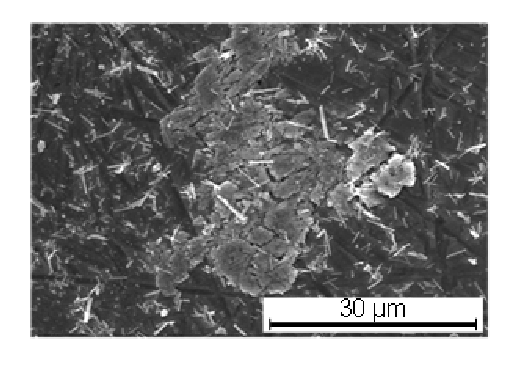
\includegraphics[scale=1.0]{slike/slika_mikroskop}
  \caption{Slika posneta z elektronskim mikroskopom \cite{Doe_1991}.} \label{fig:slika_mikroskop}
\end{centering}
\end{figure}

\begin{figure}[ht!]
\begin{centering}
  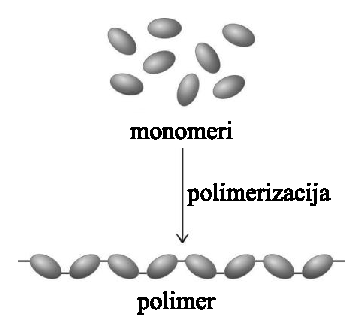
\includegraphics[scale=1.0]{slike/neke_molekule}
  \caption{Shematski prikaz postopka polimerizacije \cite{Doe_1991,Bazant_2008}.} \label{fig:neke_molekule}
\end{centering}
\end{figure}

Naslov slike z zaporedno številko slike in kratkim opisom naj bo pod sliko, sredinsko poravnan glede na sliko in besedilo. Opis slike naj se začne z veliko začetnico in zaključi s končnim ločilom. Priporočljivo je, da so imena oz. opisi slik (kot tudi preglednic) kratki, saj je iz vidika kasnejše izdelave kazala slik (oz. preglednic) to bolj primerno.\\

Slike morajo biti berljive, jasne in pregledne. Slike morajo biti dobre kvalitete in v slovenskem jeziku. Če je na sliki diagram, morajo biti veličine in enote vseh osi jasno in dosledno označene. Na mikroskopskih posnetkih mora biti ustrezno označena dolžinska skala. Slike, ki so preslikane z optičnimi bralniki, naj bodo v čim boljši ločljivosti. Slike, ki jih ustvarjate sami s programi kot so CorelDraw, Photoshop, PowerPoint idr., naj bodo shranjene v formatu *.emf (ang. Enhanced Metafile) ali *.eps (ang. Encapsulated PostScript). Na ta način bodo pri pretvarjanju dokumenta v *.pdf obliko ohranjene vse podrobnosti na sliki in tudi pri tiskanju bo zagotovljena najvišja možna kvaliteta.\\


Vsaka slika (npr. tudi sliki \ref{fig:neke_molekule} in \ref{fig:2_grafa}) naj bo smiselno umeščena v besedilo. Običajno sliko umestimo pod odstavek, v katerem jo prvič omenimo. Če sliko zaradi bolj tekočega oblikovanja besedila umestimo drugače, naj bo vsekakor umeščena v bližini prve omembe v besedilu. Če sta sliki umeščeni ena pod drugo, naj bosta med naslovom prve slike in drugo sliko 2 prazni vrstici.\\

\begin{figure}
    \begin{subfigure}[b]{.45\linewidth}
        \centering 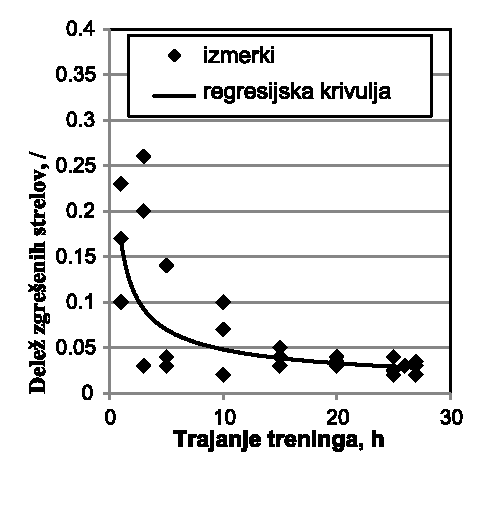
\includegraphics[scale=0.7]{slike/graf_1}
        \caption{}\label{subfig:graf1}
    \end{subfigure}%
    \quad
    \begin{subfigure}[b]{.45\linewidth}
        \centering 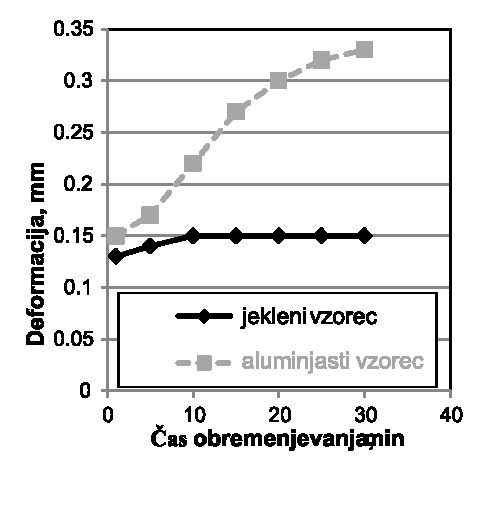
\includegraphics[scale=0.7]{slike/graf_2}
        \caption{}\label{subfig:graf2}
    \end{subfigure}

    \caption{(a) Odvisnost deleža zgrešenih strelov na tekmovanju v odvisnosti od časa treninga pred njim in (b) deformacija v odvisnosti od časa obremenjevanja za dva različna vzorca.}\label{fig:2_grafa}
\end{figure}

\begin{figure}[ht!]
\begin{centering}
  \includegraphics[scale=1.0]{slike/voda_in_nekej}
  \caption{Časovno sosledje padca projektila v vodo z višine (a) 2,1 m; in (b) 4,1 m \cite{bazant_1991}.} \label{fig:voda_in_nekej}
\end{centering}
\end{figure}

Kot je prikazano na slikah \ref{fig:2_grafa} in \ref{fig:voda_in_nekej}, lahko več povezanih diagramov združite v eno sliko, pri čemer jih jasno ločite na podsklope, t.j. (a) in (b), pri tem pa pazite na preglednost.\\

Če je slika povzeta po določenem viru, je to potrebno citirati, kot je tudi prikazano na sliki \ref{fig:slika_mikroskop}. Tudi vse slike drugih avtorjev morajo biti citirane.

\section{Enačbe}\label{sec:enacbe}

Oblikovanje enačbe je v \LaTeX u avtomatsko. Pojasnilo enačbe mora biti v tekstu.
\begin{equation}\label{eqn:e}
e = m\,c^2
\end{equation}
\begin{equation}\label{eqn:e_cel}
e_{\text{cel}}=\sum_{i=1}^{n}\,m_{i}c^2
\end{equation}
\begin{equation}\label{eqn:Nu}
N_{\text{u}} = \frac{0{,}34}{Pr_{\text{L},i}\cdot 2{,}3A}
\end{equation}

V nadaljevanju teksta, če je to potrebno, se sklicuje na ustrezno številko enačbe, npr. na enačbo (\ref{eqn:e}).\\

Za oznake veličin in druge simbole običajno uporabljamo črke latinske in grške abecede, včasih z dodatki indeksov in drugih znakov. Kot je prikazano v enačbah (\ref{eqn:e_cel}) in (\ref{eqn:Nu}), morajo biti simboli, torej oznake veličin, npr. $e$ ali $Pr$, pisane v kurzivnem (poševnem) tisku. Za simbolom ne postavljamo pike, razen če se s simbolom konča poved.\\

Indekse običajno uporabimo, kadar imata dve veličini enak simbol, ali pa če želimo veličino dodatno opredeliti (npr. $_{\text{max}}$ kot največji, $_{\text{cel}}$ kot celoten, $_{\text{z}}$ kot začetni ipd.). Indekse, ki označujejo fizikalne veličine, pišemo v kurzivnem (poševnem) tisku, opisni indeksi, ki služijo dodatnemu opredeljevanju veličin, npr. »cel« v $e_{\text{cel}}$ ali »L« v $Pr_{\text{L},i}$, pa morajo biti pisani v normalnem (pokončnem) tisku. Tudi indekse, ki so sestavljeni iz številk, pišemo v normalnem (pokončnem) tisku (npr. $A_1$), indekse iz črk, ki označujejo štetje oz. številke (npr. »i« v $m_i$ ali v $Pr_{\text{L},i}$) pa pišemo v kurzivnem (poševnem) tisku.\\

Za pravilno navajanje fizikalnih veličin, konstant, indeksov in ostalih elementov v enačbah upoštevajte »Priporočila avtorjem študijskih in strokovnih publikacij na Fakulteti za strojništvo v Ljubljani« avtorja viš. pred. dr. Stropnika \cite{stropnik_1997}.\\

\section{Citiranje in navajanje virov}\label{sec:citiranje}

Pri citiranju upoštevajte pravila citiranja, ki ne veljajo le za zaključna dela, temveč tudi v splošnem za vsako predstavitev, v kateri sta uporabljeni intelektualna ali materialna lastnina drugih avtorjev. Kot vire v čim večji meri uporabljajte \textbf{novejšo relevantno mednarodno strokovno} literaturo. Spletni viri lahko predstavljajo \textbf{največ 25 \%} vseh virov, uporabljenih v zaključnem delu.\\

Vsa uporabljena literatura se v besedilu naloge navaja sproti po zaporednih številkah v \textbf{oglatem oklepaju}, zato naj bo tudi popis bibliografije oštevilčen v skladu z zaporedjem pojavljanja citatov v dokumentu. Primeri so prikazani v naslednjih povedih:
\begin{itemize}
\item V delu Bažanta in sodelavcev \cite{bazant_1991} je podan pregled vplivov na stabilnost konstrukcij.
\item V delu Bažanta et al. \cite{bazant_1991} je podan pregled vplivov na stabilnost konstrukcij.
\item Leta 2005 sta Bažant in Cedolin \cite{bazant_1991} predstavila uporabo modalne analize pri preračunu stabilnosti konstrukcij.
\end{itemize}

Zaporedna številka vira, na katerega se sklicujemo v oglatem oklepaju, se ponovi v popisu literature (glej \ref{sec:vzorci_lit} \nameref{sec:vzorci_lit}), pri kasnejšem ponovnem sklicevanju na isto referenco pa uporabimo enako številko kot pri prvem sklicu. Vse to je v \LaTeX u avtomatsko izvedeno, vendar končna kontrola vsekakor ni odveč. \\

Popis uporabljene literature naj bo levo poravnan (ang. align left) ter oblikovan v skladu s primeri v tej predlogi (glej poglavji \ref{sec:vzorci_lit} \nameref{sec:vzorci_lit} ter 9. \refname{}) ter naj v splošnem obsega naslednje podatke:
\begin{itemize}
\item avtor, naslov dela, založba in kraj ter letnica izdaje, če gre za monografijo oz. \textbf{knjigo},
\item avtor, naslov poglavja, urednik, naslov knjige, založba, kraj in letnica izdaje ter številka začetne in zadnje strani poglavja, če gre za \textbf{poglavje v knjigi} oz. monografiji,
\item avtor, naslov članka, ime revije, številka revije, letnica izdaje ter številka začetne in zadnje strani članka, če gre za \textbf{članek} iz revije,
\item avtor, naslov prispevka, urednik ter naslov zbornika, kraj in datum konference (oz. objave zbornika) ter številka začetne in zadnje strani prispevka, če gre za \textbf{prispevek na konferenci},
\item avtor (če je naveden), naslov dela, spletni naslov, čas dostopa, če gre za vir iz \textbf{spletne strani},
\item avtor, naslov dela, tip dela, kraj in leto objave, če gre za \textbf{doktorsko disertacijo} ali drugo \textbf{zaključno delo}.
\end{itemize}

Ob sklicu na vir lahko pri več avtorjih namesto »in sodelavci« uporabimo »et al.«, na primer: V delu Bažanta et al. \cite{bazant_1991} je podan pregled vplivov\ldots\\

Vzorci popisa literature so podani v nadaljevanju. Z navedbo naštetih in (ali) drugih ustreznih podatkov pri virih, kot so na primer: referati s konferenc, patenti, standardi, predpisi, prospekti, elaborati, druge diplome, oz. pri navajanju literature upoštevajte še:
\begin{itemize}
\item SIST ISO 690: 1987(E) Documentation – Bibliographic references: Content, form and structure; ter
\item SIST ISO 690 – 2 : 1997(E) : Electronic documents or parts thereof.
\end{itemize}


\subsection{Vzorci popisa literature}\label{sec:vzorci_lit}

Za knjige:
\begin{itemize}
\item[{[1]}] Z.~P. Ba\v{z}ant, L.~Cedolin: \emph{Stability of Structures: Elastic,
  Inelastic, Fracture, and Damage Theories}. Oxford University Press, New York,
  1991.
\item[{[5]}] J.~Stropnik: \emph{Priporočila avtorjem študijskih in strokovnih publikacij
  na Fakulteti za strojništvo v Ljubljani}. Fakulteta za strojništvo,
  Ljubljana, 1997.
\end{itemize}

Za poglavja v knjigi:
\begin{itemize}
\item[{[2]}] J.~Doe: \emph{Earthquake stability}. V: Z.~P. Ba\v{z}ant, L.~Cedolin (ur.):
  \emph{Stability of Structures: Elastic, Inelastic, Fracture, and Damage
  Theories}. Oxford University Press, New York, 1991, str. 124--157.
\end{itemize}

Za revije:
\begin{itemize}
\item[{[3]}] Z.~P. Ba\v{z}ant, L.~Cedolin: \emph{Noise control}. Journal of Sound and
  Vibration \textbf{111}(2008) str. 42--50.
\item[{[4]}] J.~Gonzalez-Gutierrez, J.~L. Carillo-Estrada, J.~C. Ruiz-Suarez:
  \emph{Penetration of granular projectiles into a water target}. Scientific
  reports \textbf{4}:6762 (2014) str. 1--5.
\end{itemize}

Za konferenčne prispevke:
\begin{itemize}
\item[{[6]}] Z.~P. Ba\v{z}ant, L.~Cedolin: \emph{Modalna analiza}. V: B.~Podskrajnik (ur.):
  \emph{Kuhljevi dnevi: Zbornik referatov}. Ljubljana, Slovenija, 2005, str.
  2--5.
\item[{[7]}] Z.~P. Ba\v{z}ant, L.~Cedolin: \emph{Modal analysis}. V: S.~Smith (ur.):
  \emph{Proceedings of the 22. Congress of Polymers}. London, UK, 2007, str.
  3--8.
\end{itemize}

Za spletne vire z znanim avtorjem:
\begin{itemize}
\item[{[8]}] C.~Kogoj: \emph{Modalna analiza: izbrana poglavja iz {DTD}}. Dostopno na:
  \url{http://lab.fs.uni-lj.si/ldtd/Gradivo_za_studente/DTD/Pregled\%20teorije.pdf},\\
  Ogled: 11. 1. 2012.
\end{itemize}

Za publikacije organizacij (tiskane ali objavljene na spletnih straneh):
\begin{itemize}
\item[{[9]}] {Merkur d.d.}: \emph{Letno poročilo podjetja Merkur d.d. Kranj}, 2005.
\item[{[10]}] {Statistični urad republike Slovenije}: \emph{Statistični letopis Republike
  Slovenije 2009}. Statistični urad republike Slovenije, Ljubljana, 2009.
\item[{[11]}] {Statistični urad republike Slovenije}: \emph{Standardna klasifikacija
  dejavnosti 2005}. Dostopno na:
  \url{http://www.stat.si/klas/tabela.aspx?cvn=1895}, Ogled: 10. 1. 2012.
\end{itemize}

Za spletne strani organizacij, društev, posameznikov:
\begin{itemize}
\item[{[12]}] \emph{M Kariera – Zaposlitveni portal}. Dostopno na:
  \url{http://www.mercator.si/kariera}, Ogled: 10. 1. 2012.
\end{itemize}

Za spletne baze, enciklopedije, slovarje ipd.:
\begin{itemize}
\item[{[13]}] \emph{Engineering}. V Encyclopedia Britannica online. Dostopno na:
  \url{http://student.britannica.com/comptons/article-9274119/engineering},
  Ogled: 8. 1. 2012.
\item[{[14]}] \emph{Poslovna aplikacija}. V eSlovarju. Dostopno na:
  \url{http://www.eslovar.com/besedilo.asp?id=1563}, Ogled: 8. 1. 2012.
\end{itemize}

Za zakonodajo (uradni listi, pravilniki, standardi):
\begin{itemize}
\item[{[15]}] \emph{Zakon o gospodarskih družbah}, {U}radni list RS št. 42/2006, 60/2006
  popr., 26/2007-ZSDU-B, 33/2007-ZSReg-B, 67/2007-ZTFI (100/2007 popr.),
  10/2008, 68/2008, 23/2009; Odl. US: U-I-268/06-35.
\item[{[16]}] \emph{Zakon o okoljskih predpisih}, {U}radni list RS št. 72/2009-UPB2,
  65/2010.
\item[{[17]}] {ISO 2573:1977}: \emph{Tensile testing systems – Determination of K-value}.
\item[{[18]}] {DIN 4768:1990}: \emph{Determination of surface roughness values R$_a$, R$_z$,
  R$_{max}$}.
\item[{[19]}] {JIS B 0601:2001}: \emph{Geometrical product specifications (GPS) profile
  method – Terms, definitions and surface texture parameters}.
\end{itemize}

Za doktorske disertacije in druga zaključna dela:
\begin{itemize}
\item[{[20]}] A.~Novak: \emph{Izdelava avtomatiziranega stroja za lupljenje krompirja}:
  \emph{Doktorska disertacija}, Univerza v Ljubljani, 2015.
\end{itemize}

Popis literature je v \LaTeX u izveden avtomatsko, glede na vašo bazo bibliografij (ki se v primeru predloge nahaja na References.bib) ter izbrane makre, ki ustrezno generirajo \TeX~sintakso bibliografije. Za zaključna dela na Fakulteti za Strojništvo je izdelan ustrezen makro, ki se nahaja v fs\_zakljucne\_naloge.bst. Uporabo le-tega definirate z ukazom \verb|\bibliographystyle{fs_zakljucne_naloge}| v glavni datoteki.\\

Sklici na popis literaturo so avtomatsko generirani, npr: \cite{bazant_1991}, \cite{Doe_1991},  \cite{Bazant_2008}, \cite{Gonzalez_2014, Bazant_2005} \cite{Bazant_2007, Kogoj_DTD, Merkur_2005, SURS_2009, SURS_2005, MKariera, Encyclopedia, Posl_app, ZGD, ZOP}, \cite{ISO_2573}, \cite{DIN_4768}, \cite{DIN_4768} in \cite{JISB0601, Novak_2015}.






\newpage

% !TeX spellcheck = si_SI
\chapter{Namen in cilji doktorske naloge}\label{cha:namen}

\section{Predstavitev problema}\label{sec:predstavitev_problema}
Na tem mestu na podlagi predstavljenega \emph{Stanja razvoja} povzemite dosedanje ključne izsledke in ugotovitve, predvsem pa odprta vprašanja in problematiko, ki do tega trenutka še niso bili razrešeni.

\section{Teza in cilji}\label{sec:teza}
V tem poglavju predstavite raziskovalno hipotezo, ki ste jo postavili ob pregledu \emph{Stanja razvoja} in vam je služila kot izhodišče za zasnovo doktorskega dela. Predstavite konkretne cilje, ki jih boste v povezavi z raziskovalno hipotezo v okviru doktorskega dela skušali doseči in ki bodo torej neposredno predstavljali prispevek znanosti ali tudi širše. Pišite, kaj boste delali, kaj pričakujete od teoretičnih in kaj od praktičnih raziskav ter kakšna so tveganja in nevarnosti, da teh ciljev ne boste dosegli. Pišite o hipotezah in ne o dobljenih rezultatih.

\section{Potek dela}\label{sec:potek}
V tem delu se osredotočite na to, kako je delo strukturirano (po poglavjih), torej npr. kje je predstavljen nek vsebinski sklop in kako so posamezni vsebinski sklopi med seboj povezani.

\section{Publikacije}\label{sec:publikacije}
V primeru, da so bili rezultati doktorskega dela objavljeni ali pripravljeni kot celovite znanstvene publikacije, lahko v tem podpoglavju navedete seznam objavljenih publikacij. Predstavitev publikacij (seznam) je prostovoljna rubrika.
\newpage

% !TeX spellcheck = si_SI
\chapter{Metodologija raziskave}\label{cha:metodologija}

V tem poglavju glede na tip doktorskega dela (raziskovalni ali razvojni) predstavite, razložite in utemeljite uporabljene \textbf{metode oz.\ postopke} meritev, izračunov, modelirnih postopkov itn. ter predstavite in utemeljite izbor uporabljenih \textbf{materialov in vzorcev}. V tem poglavju posebej razdelajte tudi merilno negotovost.

\section{Preračuni}\label{sec:preracuni}

Na podlagi predpostavk o \ldots smo za preračun \ldots uporabili izpeljavo Bažanta et al.\ \cite{Bazant_2008} \ldots Lorem ipsum dolor sit amet, consectetur adipiscing elit, sed do eiusmod tempor incididunt ut labore et dolore magna aliqua. Ut enim ad minim veniam, quis nostrud exercitation ullamco laboris nisi ut aliquip ex ea commodo consequat. Duis aute irure dolor in reprehenderit in voluptate velit esse cillum dolore eu fugiat nulla pariatur. Excepteur sint occaecat cupidatat non proident, sunt in culpa qui officia deserunt mollit anim id est laborum.

\section{Eksperimentalni del}\label{sec:eksperiment}
\subsection{Vzorci in materiali}\label{sec:vzorci}
\subsubsection{Zobniški par}\label{sec:zobniski_par}
Za zobniški par smo izbrali \ldots Lorem ipsum dolor sit amet, consectetur adipiscing elit, sed do eiusmod tempor incididunt ut labore et dolore magna aliqua. Ut enim ad minim veniam, quis nostrud exercitation ullamco laboris nisi ut aliquip ex ea commodo consequat. Duis aute irure dolor in reprehenderit in voluptate velit esse cillum dolore eu fugiat nulla pariatur. Excepteur sint occaecat cupidatat non proident, sunt in culpa qui officia deserunt mollit anim id est laborum.

\subsubsection{Gred}\label{sec:gred}
Gred je bila izdelana iz \ldots Lorem ipsum dolor sit amet, consectetur adipiscing elit, sed do eiusmod tempor incididunt ut labore et dolore magna aliqua. Ut enim ad minim veniam, quis nostrud exercitation ullamco laboris nisi ut aliquip ex ea commodo consequat.


\subsection{Metodologija preizkusov}\label{sec:metodologija}
\subsubsection{Zobniško preizkuševališče}\label{sec:zobn_experiment}
Zasnovali smo \ldots Lorem ipsum dolor sit amet, consectetur adipiscing elit, sed do eiusmod tempor incididunt ut labore et dolore magna aliqua. Ut enim ad minim veniam, quis nostrud exercitation ullamco laboris nisi ut aliquip ex ea commodo consequat. Duis aute irure dolor in reprehenderit in voluptate velit esse cillum dolore eu fugiat nulla pariatur. Excepteur sint occaecat cupidatat non proident, sunt in culpa qui officia deserunt mollit anim id est laborum.

Lorem ipsum dolor sit amet, consectetur adipiscing elit, sed do eiusmod tempor incididunt ut labore et dolore magna aliqua. Ut enim ad minim veniam, quis nostrud exercitation ullamco laboris nisi ut aliquip ex ea commodo consequat. Duis aute irure dolor in reprehenderit in voluptate velit esse cillum dolore eu fugiat nulla pariatur. Excepteur sint occaecat cupidatat non proident, sunt in culpa qui officia deserunt mollit anim id est laborum.

\subsubsection{Merilnik pomikov (LVDT)}\label{sec:LVDT}
Za merjenje \ldots smo uporabili linearno variabilni diferencialni transformator (LVDT), s čimer smo zagotovili \ldots Lorem ipsum dolor sit amet, consectetur adipiscing elit, sed do eiusmod tempor incididunt ut labore et dolore magna aliqua. Ut enim ad minim veniam, quis nostrud exercitation ullamco laboris nisi ut aliquip ex ea commodo consequat. Duis aute irure dolor in reprehenderit in voluptate velit esse cillum dolore eu fugiat nulla pariatur. Excepteur sint occaecat cupidatat non proident, sunt in culpa qui officia deserunt mollit anim id est laborum.

\subsection{Analiza deformacijskih mehanizmov}\label{sec:def_mehanizmi}
Po preizkusih smo površine analizirali z \ldots Lorem ipsum dolor sit amet, consectetur adipiscing elit, sed do eiusmod tempor incididunt ut labore et dolore magna aliqua. Ut enim ad minim veniam, quis nostrud exercitation ullamco laboris nisi ut aliquip ex ea commodo consequat.

\section{Korelacija preračunov in eksperimentalnih rezultatov}\label{sec:korelacija}
Lorem ipsum dolor sit amet, consectetur adipiscing elit, sed do eiusmod tempor incididunt ut labore et dolore magna aliqua. Ut enim ad minim veniam, quis nostrud exercitation ullamco laboris nisi ut aliquip ex ea commodo consequat. Duis aute irure dolor in reprehenderit in voluptate velit esse cillum dolore eu fugiat nulla pariatur. Excepteur sint occaecat cupidatat non proident, sunt in culpa qui officia deserunt mollit anim id est laborum.

Lorem ipsum dolor sit amet, consectetur adipiscing elit, sed do eiusmod tempor incididunt ut labore et dolore magna aliqua. Ut enim ad minim veniam, quis nostrud exercitation ullamco laboris nisi ut aliquip ex ea commodo consequat. Duis aute irure dolor in reprehenderit in voluptate velit esse cillum dolore eu fugiat nulla pariatur. Excepteur sint occaecat cupidatat non proident, sunt in culpa qui officia deserunt mollit anim id est laborum.



\newpage


% !TeX spellcheck = si_SI
\chapter{Rezultati}\label{cha:rezultati}

V tem poglavju predstavite \textbf{ugotovljena dejstva}, torej rezultate vaših meritev, analiz, preračunov ipd. Če je naloga obsežnejša in sestavljena iz več ločenih sklopov, lahko rezultate iz posameznega sklopa predstavljate tudi v ločenih (pod)poglavjih. Končna oblika mora biti takšna, da je karseda pregledna, jasna in razumljiva.
\newpage


% !TeX spellcheck = si_SI
\chapter{Diskusija}\label{cha:diskusija}

V tem delu predstavite vaše razumevanje oz. \textbf{razlago} rezultatov in komentar. Zaželeno je, da so rezultati in diskusija o rezultatih predstavljeni ločeno. V diskusiji pojasnite pomen rezultatov tako, da rezultate argumentirano (citiranje referenc) primerjate z doslej znanimi in razložite ključne ugotovitve, ki nadgrajujejo doslej poznano stanje na danem področju raziskav, s čimer pojasnite doprinos doktorskega dela k znanosti. Končna oblika mora biti takšna, da je karseda pregledna, jasna in razumljiva.
\newpage

% !TeX spellcheck = si_SI
\chapter{Zaključki}\label{cha:zakljucki}

V zaključku opišite glavne rezultate in ugotovitve, ki jih povzamete v nekaj (oštevilčenih) točkah. Pazite, da zaključek ne bo ponovitev uvoda. Tukaj opišite oz.\ povzemite izključno tisto, kar je bilo narejeno in ugotovljeno. Jezikovno lahko zaključke oblikujete na naslednji način, vendar je slog podajanja zaključkov prepuščen presoji avtorja:
\begin{enumerate}
\item Izmerili smo / Zasnovali smo \ldots
\item Pokazali smo \ldots
\item Dobljeni rezultati pomenijo \ldots
\item Ugotovili smo \ldots
\item \ldots
\item \ldots
\end{enumerate}

 
\newpage

\bibliographystyle{fs_zakljucne_naloge}
%\bibliographystyle{unsrt}
%\bibliographystyle{unifs}
\bibliography{References}
\addcontentsline{}{chapter}{Literatura}
\newpage

% !TeX spellcheck = si_SI
\chapter{Priloga A}\label{cha:priloga}
Prilogo je lahko dodana le izjemoma. Vsebuje naj takšne informacije, ki so sicer potrebne za prikaz celovitosti, bi pa motile osnovno poročilo, ker bi bralcu odvračale pozornost od osnovne teme. Sem spadajo npr. daljša izvajanja enačb, numerični izračuni, ponavljajoči se diagrami, iztiski programov in drugo. 
\newpage
\thispagestyle{empty}
\mbox{}

\end{document} 